\section{Unabhängige Ereignisse}
%\textbf{Definition}: ER. A und B heißen unabhängig, wenn $$\mathds{P}[A\cap B] = \mathds{P}[A] - \mathds{P}[B]$$
%A, B unabhängig $\Rightarrow$\\
%$\mathds{P}[A\vert B] = \mathds{P}[A]$\medskip\\
%\textbf{Bsp.}:\\
%1 fairer Würfel\\
%A= ''gerade Zahl gewürfelt'' = \{2,4,6\}\\
%B = ''Augenzahl $\geq$ 5'' = \{5,6\}\medskip\\
%$\mathds{P}[A] = \frac{1}{2}..:$
Zwei Formeln:
\begin{enumerate}
	\item $\mathds{P}[A\cup B] = \mathds{P}[A]+\mathds{P}[B] \quad$, falls A $\cap$ B = $\emptyset$
	\item $\mathds{P}[A\cap B] = \mathds{P}[A]*\mathds{P}[B] \quad$, falls A und B unabh.
\end{enumerate}
\textbf{Bem.}: Disjunkt und unabh sind verschiedene Begriffe.\\
Seien A, B disj, d.g. A $\cap$ B = $\emptyset$ $\Rightarrow \mathds{[\underbrace{A \cap B}_\emptyset]}= 0 \neq \mathds{P}[A]*\mathds{P}[B]$\\$\Rightarrow$ A und B abh. (Falls $\mathds{P}[A], \mathds{P}[B] \neq 0$\medskip\\
\textbf{Definition}\\
Ereignisse A,B,C heißen
\begin{itemize}
	\item paarweise unabh, wenn $\mathds{P}[A\cap B] = \mathds{P}[A]*\mathds{P}[B],\: \mathds{P}[A\cap C] =$\\$ \mathds{P}[A]*\mathds{P}[C],\:\mathds{P}[B \cap C]=\mathds{P}[B]*\mathds{P}[C]$
	\item unabh, wenn zusätzlich: $\mathds{P}[A\cap B \cap C] = \mathds{P}[A]*\mathds{P}[B]*\mathds{P}[C] \quad \text{unabh } \Rightarrow \text{ paarweise unabh}$
\end{itemize}
\textbf{Bsp.}: 3 Ereignisse, die paarweise unabh, aber nicht unabh.\\
3 Würfel: $x_1,x_2,x_3$ seien die 3 Augenzahlen
\\$A = ''x_1 = x_2'' \quad B = ''x_2 = x_3'' \quad C = ''x_3 = x_1''$\smallskip\\
$\Omega = \{1,...,6\}^3 = \{(a,b,c):a,b,c \in \{1,...,6\}\} \quad \# \Omega = 6^3$\smallskip\\
$A = \{(a,a,c):a,c \in \{1,...,6\}\}  \quad C = \{(a,b,a):a,b\in \{1,..,6\}\} $\\
$B = \{(a,b,b,): a,b \in \{1,...,6\}\}$\\$\#A=6^2\quad \# B= 6^2 \quad \#C=6^2$\medskip\\
$\mathds{P}[A] = \mathds{P}[B]=\mathds{P}[C]=\dfrac{6^2}{6^3} = \dfrac{1}{6}$\\
\textbf{Beh.}: A, B, C sind paarweise unabh. Wir zeigen: $\mathds{P}[A \cap B] = \mathds{P}[A] * \mathds{P}[B]$\smallskip\\
$A \cap B = ''x_1 = x_2, x_2 = x_3'' = ''x_1 = x_2 =x_3'' = \{(a,a,a):a \in \{1,...,6\}\} $\\$ \#(A\cap B) = 6$\smallskip\\
$\mathds{P}[A\cap B] = \dfrac{6}{6^3} = \dfrac{1}{6^2} = \dfrac{1}{6}* \dfrac{1}{6}= \mathds{P}[A]*\mathds{P}[B] \Rightarrow \text{ A und B unabh}$\medskip\\
\textbf{Beh.}: A,B,C sind abh. \\$A \cap B \cap C = ''x_1 = x_2, x_2 =x_3, x_3 = x_1'' = ''x_1 = x_2 =x_3'' \quad \#(A\cap B \cap C) = 6$\smallskip\\
$\mathds{P}[A \cap B \cap C]= \dfrac{6}{6^3} = \dfrac{1}{6^2} \neq \mathds{P}[A]*\mathds{P}[B]*\mathds{P}[C] \Rightarrow A,B,C \text{abh.}$
\subsection{Eigenschaften von unabhängig}
Seien A,B unabhängige Ereignisse. Dann sind
\begin{itemize}
	\item $A \text{ und } B^C \text{ unabh}$
	\item $A^C \text{ und } B \text{ unabh}$
	\item $A^C \text{ und } B^C \text{ unabh}$
\end{itemize}
\textbf{Bew.}: Wir zeigen $A \text{ und } B^C$ sind unabh
\begin{tabbing}
	$\mathds{P}[A\cap B^C] =$\=$ \mathds{P}[A]-\mathds{P}[A\cap B]\underset{\text{A, B unabh}}{=}\mathds{P}[A] - \mathds{P}[A]*\mathds{P}[B]$\\
	\>$\mathds{P}[A]*(1.\mathds{P}[B])=\mathds{P}[A]*\mathds{P}[B^C] \Rightarrow A, B^C $ unabh \qed
\end{tabbing}
Weitere \textbf{Beh.}: Seien A,B,C unabh. Dann sind:
\begin{itemize}
	\item A,B $\cup$ C unabh 
	\item A, B $\cap$ C unabh
	\item A, B $\Delta$ C unabh
\end{itemize}
\textbf{Bsp.}: Zuverlässigkeit: System besteht aus \textbf{n} Komp. 1,...,n\\
Wkeit, dass Komp \textbf{i} ausfällt ist $\mathds{P}[A_i]=p_i$
\begin{enumerate}
	\item [a)] Parallelschaltung 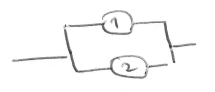
\includegraphics[width=0.3\textwidth]{img/parallel.PNG} \\
	$\mathds{P}[\text{Ausfall des Systems}] = \mathds{P}[A_1\cap A_2] = p_1p_2$
	\item [b)] Reihenschaltung 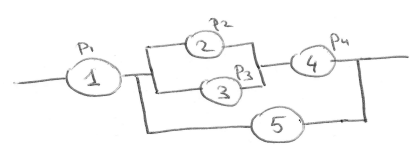
\includegraphics[width=0.3\textwidth]{img/reihe.PNG}\\
	$\mathds{P}[\text{Ausfall des Systems}]= \mathds{P}[\underbrace{A_1 \cup A_2}_{\substack{\text{nicht disj,}\\\text{unabh}}}] = 1-\mathds{P}[(A_1 \cup A_1)^C]\overset{\text{de Morgan}}{=}$\smallskip\\
	$1-\mathds{P}[\underbrace{A_1^C \bigcap A_2^C}_\text{unabh}]$\smallskip\\
	$=1.\mathds{P}[A_1^C]*\mathds{P}[A_2^C]$\smallskip\\
	$=1-(1-p_1)(1-p_2)=p_1+p_2 - p_1p_2$\medskip\\

	$\mathds{P}[\text{Ausfall}] = ? $
\end{enumerate}
Ereignis, dass das System ausfällt:\\
A = Ausfall des Systems = $A_1 \cup (A_5\cap (A_4 \cup (A_2 \cap A_3)))$\smallskip\\
$\mathds{P}[A] = ?$\\
$\mathds{P}[\text{2 und 3 fällt aus}] = p_2p_3$\smallskip\\
$\mathds{P}[\text{2,3,4 fällt aus}] = p_2p_3+p_4 -p_2p_3p_4$\smallskip\\
$\mathds{P}[\text{2,3,4,5 fällt aus}] = (p_2p_3+p_4-p_2p_3p_4)p_5$\smallskip\\
$\mathds{P}[A] = p_1 + p_\text{Rest} - p_1p_\text{Rest} =$ ... Prof sagt trivial \qed\medskip\\
\textbf{Def.}: n Ereignisse $A_1, A_2,...,A_n$ sind
\begin{itemize}
	\item paarweise unabh, wenn $\mathds{P}[A_i \cap A_j] = \mathds{P}[A_i] * \mathds{P}[A_j] \forall i \neq j$
	\item unabh, wenn: $\forall m \in \{2,...,n\} \: \forall 1 \leq i_1 < i_2 <...<i_m\leq n$
	$$\mathds{P}[A_{i1}\cap A_{i2}\cap ... \cap A_{im}] = \mathds{P}[A_{i1}* ... * \mathds{P}[A_{im}]$$
	(D.h. Produktformel gilt für alle Teilfamilien)
\end{itemize} 
\textbf{Beh.}: Blockungslemma\\
\textbf{Bsp.}: Seien A,B,C,D,E,F,G unabh. Er.
$$(A \Delta C) \cap E^C \cup C, \: B^C\cap F,\: D\cup G \quad \text{unabh}$$ 
$$\text{Aber:} \quad A \Delta \mathbf{C} \text{ und } B \cup \mathbf{C} \text{ sind im Allgemeinen abgh.}$$
\textbf{Bem}: $\Omega$ und A sind immer unabh. \hspace{1cm} $\mathds{P}[\Omega \cap A] = \mathds{P}[A]=\mathds{P}[\overbrace{\Omega}^1]*\mathds{P}[A]$\\
$\emptyset$ und A sind immer unabh \hspace{1cm} $\mathds{P}[\emptyset \cap A] = \mathds{P}[\emptyset]=0=\mathds{P}[\emptyset]*\mathds{P}[A]$
\chapter{Satz von Bayes}
\subsubsection{Satz: Formel der totalen Wkeit}
Sei $\Omega = B_1  \dot{\cup} ... \dot{\cup} B_n $ disj. Zerlegung von $\Omega$, d.h. $B_i \cap B_j = \emptyset \: \forall i \neq j$ und $\Omega = B_1 \cup ...\cup B_n$\\
Sei $\mathds{P}[B_i] \neq 0 \forall i$\medskip\\
Sei A $\subset$ $\Omega$ ein weiteres Er. Dann gilt: 
$$\mathds{P}[A] = \mathds{P}[B_1]*\mathds{P}[A \vert B_1] + \mathds{P}[B_2]*\mathds{P}[A\vert B_2]+...$$
\textbf{Beweis}: $\mathds{P}[A] = \mathds{P}[A\cap B_1]+\mathds{P}[A \cap B_2] +.....= \mathds{P}[B_1]*\mathds{P}[A \vert B_1] + \mathds{P}[B_2]*\mathds{P}[A\vert B_2]+... $\qed\medskip\\
\textbf{Beispiel}: Population Personen: krank und gesund\\
1\% der Population ist krank.\medskip\\
\begin{tabbing}
	Schnelltest: \= Bei einer Kranken Person mit Wkeit 90\% positiv.\\
	\> Bei einer gesunden Person mit Wkeit 20\% positiv
\end{tabbing}
A= ''Test ist Positiv''\hspace{1cm} $\mathds{P}[A]= 0,001*0.9+0,99*0,2 = 0,207$\smallskip\\
Lösung mit der Formel\\
$B_1 $ = ''Person krank'' \hspace{1cm} $B_2$ = ''Person gesund''\\
$ \mathds{P}[B_1]=0,01 \Rightarrow  \mathds{P}[B_2] =0,99$\smallskip\\
$\mathds{P}[A \vert B_1] = 0,9 \qquad [\text{nicht } \mathds{P}[A\cap B_1]$\smallskip
$\mathds{P}[A\vert B_2] = 0,2$\smallskip\\
$\mathds{P}[A] = \mathds{P}[B_1]*\mathds{P}[A\vert B_1] + \mathds{P}[B_2]*\mathds{P}[A\vert B_2]$\smallskip\\
$=0,01*0.9+0.99*0,2$\medskip\\
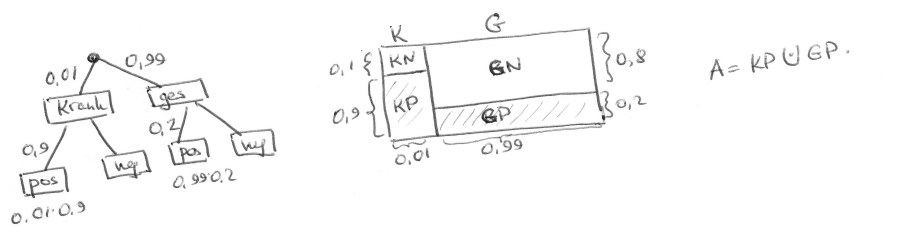
\includegraphics[width=0.9\textwidth]{img/baum.PNG}\\